\chapter{Results and Discussions} \label{chap:results}


	This chapter presents the applications. {\textcolor{red}{Write intro. Describe problems in more detail}}
	
	\section{GEM - Phase Field Coupling}
The objective of {\YJ} development was to allow concurrent coupling of GEM with the phase field module in MOOSE. To achieve this a two step process was adopted. The first step was an offline coupling where GEM calculations are used to pre tabulate the Gibbs energy and chemical potential data. The data is then used to generate interpolated functions using the \texttt{PiecewiseLinearInterpolationMaterial} object in MOOSE. The next step was to move towards a full coupling for which a UserObject has been developed and is currently being tested. The UserObject will allow direct incorporation of GEM calculation in the phase field module and other codes. A phase field simulation was performed at the University of Florida\footnote{The phase field calculations were performed by Chaitanya Bhave, University of Florida.} to demonstrate the current capabilities. In the model, the corrosion of \ce{Ni} metal by a \ce{LiF-NiF2} salt at 1150\si{\kelvin} was simulated with values for the Gibbs energy supplied by the Gibbs energy minimiser. As shown in figure~\ref{fig:pfgibbs}, the use of GEM allows capturing the excess mixing effects which were not captured by the dilute solution Nernst model used previously. Since the excess energies can have significant contributions for larger systems such as ones with impurities, being able to capture the additional contributions can significantly improve the fidelity.
    \begin{figure}[h!]
        \centering
        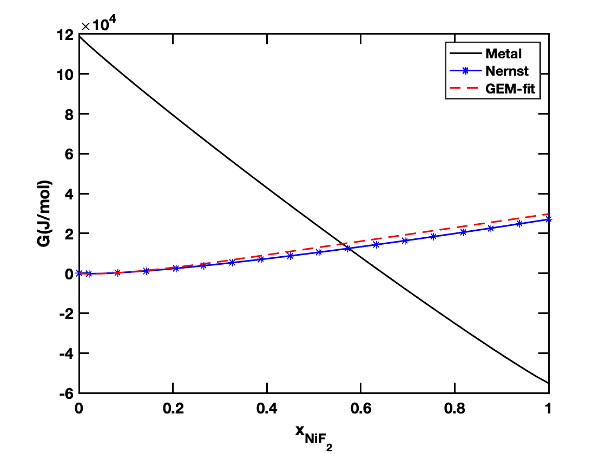
\includegraphics[width=0.75\textwidth]{figures/chapter-7/gibbs.png}
        \caption{Comparison of Gibbs energy predicted by the Gibbs energy minimiser vs. the dilute Nernst energy model used previously.}
        \label{fig:pfgibbs}
    \end{figure}

The result of \ce{Ni} leaching into the molten salt has been shown in figure~\ref{fig:pfres}. In the simualtion, the corrosion of \ce{Ni} by \ce{LiF-NiF2} was simulated under oxidising conditions. The mole fraction of \ce{Ni} in the molten salt phase was fixed as $x_{\ce{Ni}} = 0.001$.
\begin{figure}[h!]
        \centering
        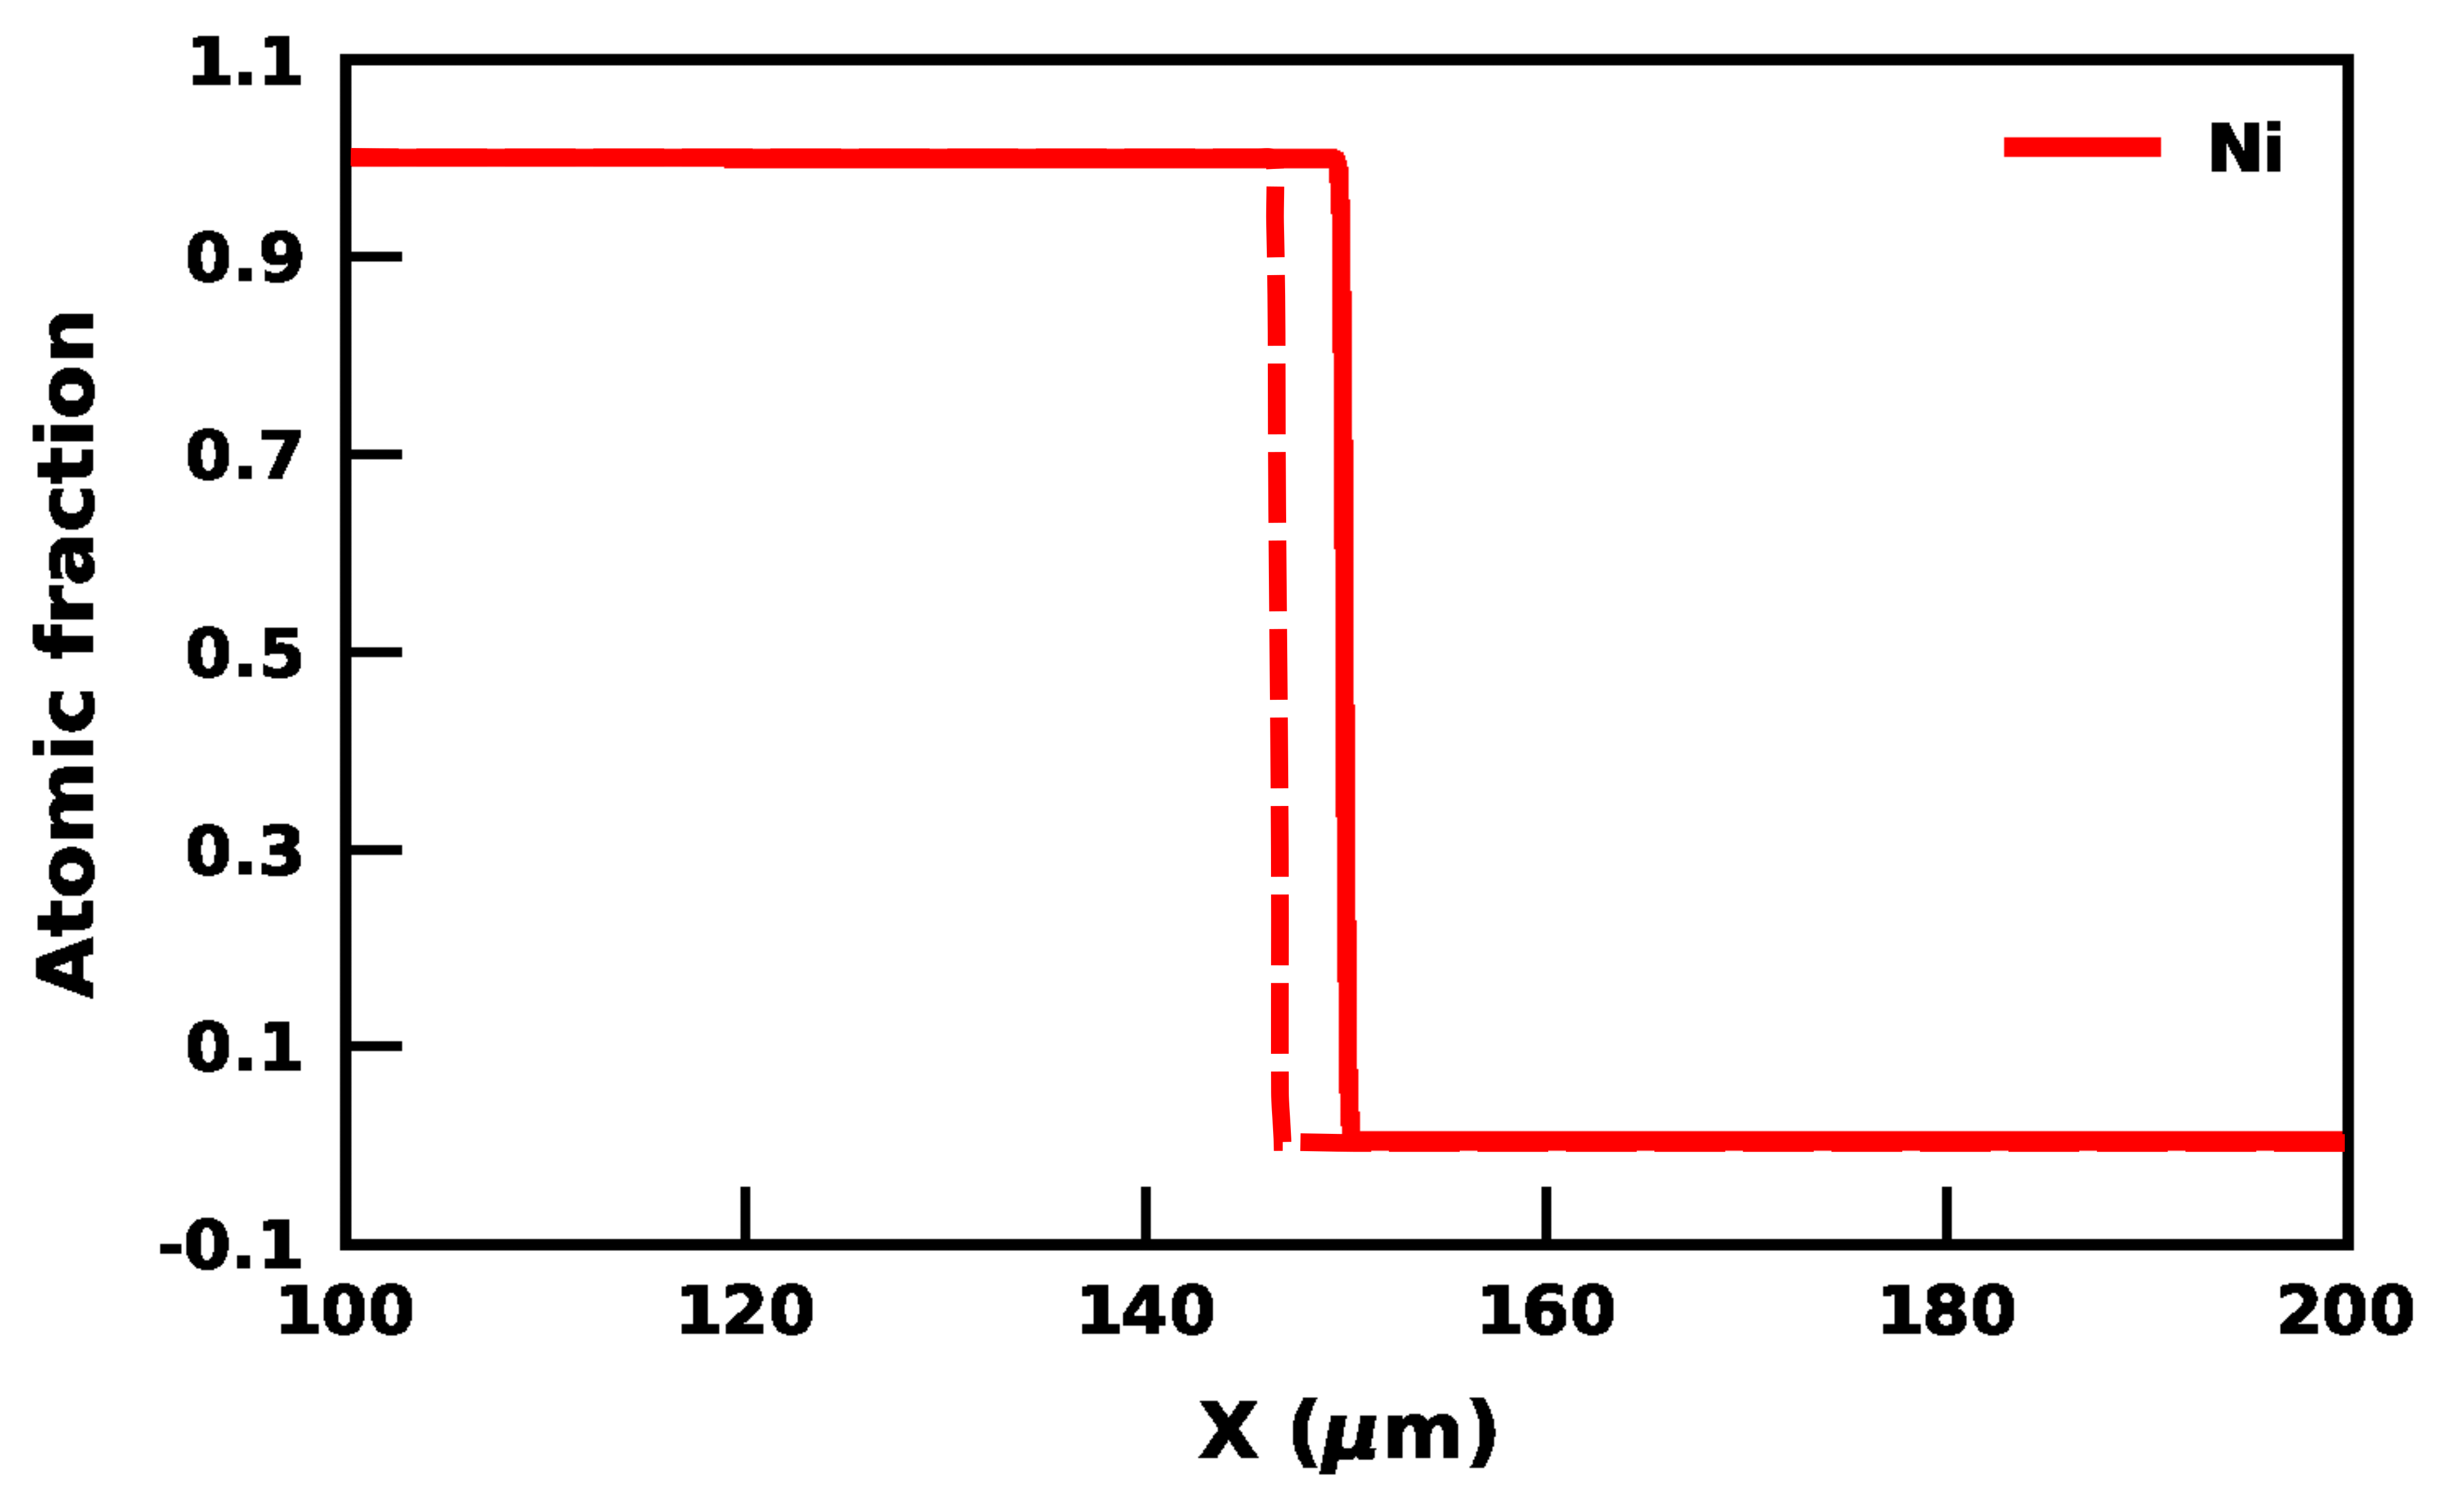
\includegraphics[width=0.75\textwidth]{figures/chapter-7/pfres.png}
        \caption{Simulation of \ce{Ni} corrosion by \ce{LiF-NiF2} salt. Initially, the domain contained \ce{Ni} in the left half of the domain and molten salt in the right half with the interface shown by the solid vertical line at the centre of the domain. At the end of the simulation, denoted by the dashed vertical line, the oxidising conditions lead to the leaching of \ce{Ni} from the metal into the molten salt as exhibited by the interface shifting to the left.}
        \label{fig:pfres}
    \end{figure}
       
\subsection{Phase Equilibrium Calculations}
    To demonstrate the capabilities of {\GEM}, the \ce{NaF-CsF} binary system was selected. This system has been recently re-evaluated experimentally by Lipkina \textit{et al.} \cite{Lipkina:2022aa} and the phase diagram was reproduced using {\GEM} and compared to the experimental results. The calculations from {\YJ} are shown in figure~\ref{fig:res_phased} and show excellent agreement with the experimental data for the eutectic points. There is, however, a departure between the liquidus points calculated by Lipkina \textit{et al.} and the ones predicted by {\YJ}. This is a direct consequence of the database used in the calculations as it has not been updated to reflect the recent experimental results. In fact, as shown by the solid black line, the calculations match the results of the previously available experimental data. The example not only highlights the capability of {\GEM} but also shows a need for the re-evaluation of the \ce{NaF-CsF} thermodynamic model currently used in the databases.
\begin{figure}
         \centering
         \includegraphics[width=0.8\textwidth]{figures/chapter-7/phasedia.png}
 	 \caption{Yellowjacket prediction of \ce{NaF-CsF} phase diagram with the original phase diagram overlayed on top.}
	 \label{fig:res_phased}
\end{figure}
    
\begin{figure}
         \centering
         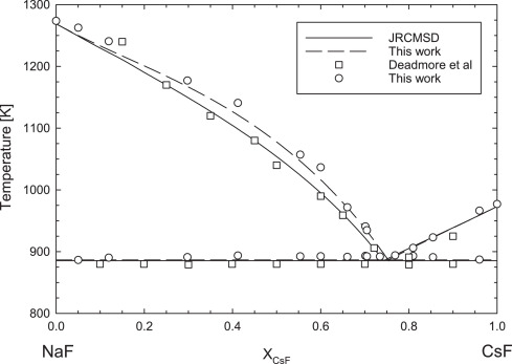
\includegraphics[width=0.7\textwidth]{figures/chapter-7/pdo.png}
         \caption[Reference \ce{NaF-CsF} phase  diagram from Lipkina \textit{et al.}]{Reference \ce{NaF-CsF} phase  diagram from Lipkina \textit{et al.} \cite{Lipkina:2022aa}.}
     \label{fig:res_refdia}
\end{figure}
 
\subsection{Vapour Pressure in MSR}
    Another demonstration of capabilities of GEM focuses on the change of vapour pressure of elements in gas phase and the element potential evolution in MSR. For the purpose of demonstration, a fictive system representative of a molten salt system (\ce{FLiBe}) with some dissolved fissile material (\ce{U}) and some fission products (\ce{Nd, Ce, La, Cs, Rb}) was simulated to undergo an unmitigated increase in temperature. Such a scenario can be relevant in source term analyses and is of particular interest for MSR design and deployment. The predicted vapour pressures are shown in figure~\ref{fig:res_vpmsr} and the predicted element potentials are shown in figure~\ref{fig:res_epmsr}. One must note that the results are purely for capability demonstration and must not be treated as physically relevant. However, they do exhibit cases where one might find the use of {\GEM} relevant.
  
\begin{figure}
     \centering
     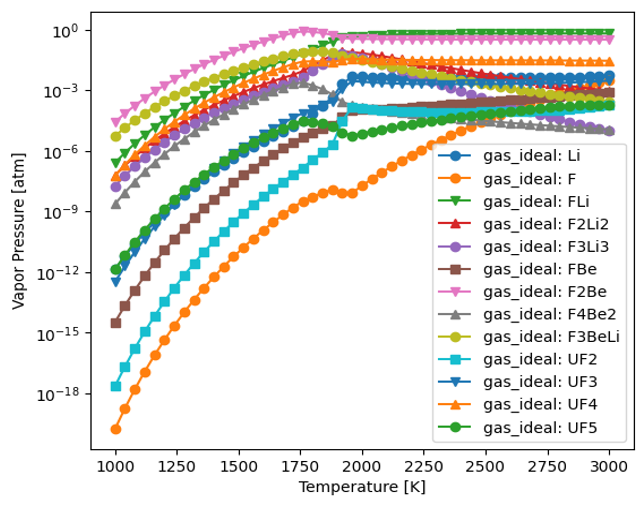
\includegraphics[width=0.7\textwidth]{figures/chapter-7/vp_msr.png}
     \caption{Vapour pressure prediction in molten salt system.}
     \label{fig:res_vpmsr}
\end{figure}

\begin{figure}
         \centering
         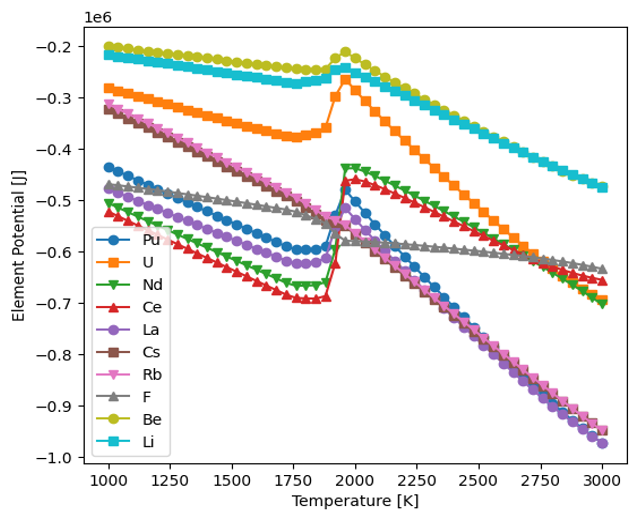
\includegraphics[width=0.7\textwidth]{figures/chapter-7/ep_msr.png}
         \caption{Element potential evolution in MSR.}
         \label{fig:res_epmsr}
 \end{figure}
 
\section{Verification}
To ensure that accuracy of results, a significant effort was put into verification of {\YJ}-GEM results by comparison with commercial code FactSage. For this, a representative system was selected (the system composition is the same as that used by Poschmann \textit{et al.} \cite{Poschmann:2021ab}) and the relative difference of the mole fractions of each quadruplet was compared between {\YJ} and FactSage. As shown in figure~\ref{fig:verif}, the results are in excellent agreement with FactSage and the maximum relative difference is of the order of $1e-5$.
 \begin{figure}[h!]
        \centering
        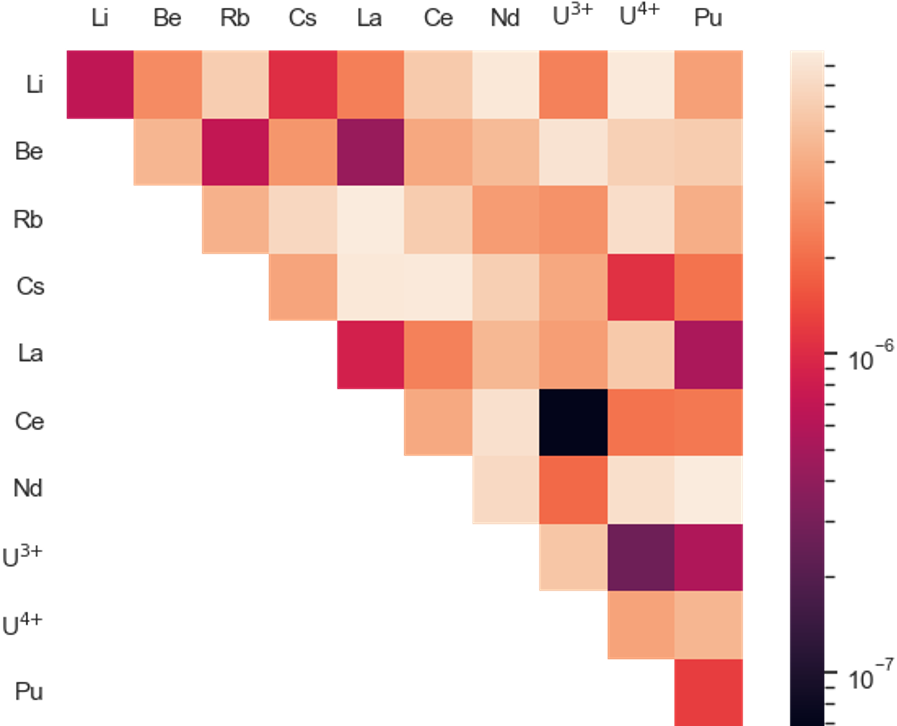
\includegraphics[width=0.75\textwidth]{figures/chapter-7/verif.png}
        \caption{Relative difference of mole fraction of quadruplets when compared to FactSage}
        \label{fig:verif}
    \end{figure}